\documentclass[10pt, a5paper, twoside]{NGPLS}
\author{周造麟}
\title{30 天 LaTeX}

%\usepackage{luatexja-fontspec}
%\setmainjfont{jf-openhuninn-1.1.ttf}
\usepackage{xeCJK}
\setCJKmainfont{jf-openhuninn-1.1.ttf}

\setlength{\parindent}{0pt}
\linespread{1.35}
\pagenumbering{arabic}

\usepackage[pipeTables, strikeThrough = true]{markdown}
\markdownSetup{fencedCode = true}
\markdownSetup{
  renderers = {
    image = {\begin{figure}[!htb]
      \centering
      \includegraphics[width = .8\linewidth]{#3}%
      \ifx\empty#4\empty\else
        \caption{#4}\label{fig:#1}%
      \fi
    \end{figure}},
    }
}
\usepackage{graphicx}
\graphicspath{{fig/}}

\usepackage{etoolbox}
%\AtBeginEnvironment{itemize}{\vskip6pt}
\AtBeginEnvironment{tabular}{\vskip6pt}
\AfterEndEnvironment{tabular}{\vskip6pt}

\usepackage[svgnames]{xcolor}
%\definecolor{LightGray}{gray}{0.9}

\usepackage{minted}
%\usemintedstyle{borland}

\usepackage{xurl}
\usepackage[breaklinks=true]{hyperref}
\urlstyle{same}
\hypersetup{
colorlinks=true,
linkcolor=blue,
urlcolor=cyan,
hyperindex = false
}

%\setlength{\parskip}{0.1\baselineskip}

\usepackage{amsmath}
\usepackage{amsfonts}
\usepackage{amssymb}

\usepackage{geometry}
\geometry{top=1.5cm, outer=1.75cm, inner=1.5cm, bottom=1.5cm, footskip=24pt}

\begin{document}%\color{Gold}\pagecolor{black}
\maketitle
\tableofcontents\newpage
\begin{markdown}
#30天 LaTeX 挑戰 Day 1 編譯引擎、格式、發行版與編輯器(上)

------

##巨集

巨集是指將一連串的指令換為以一串文字替代,類似將往(往前+右轉)X4 換成話正方形一樣,LaTeX 有許多的巨集包(以下用 Package 代稱)可供使用,如有特殊需求也可以自行撰寫。

##編譯引擎與格式的差異

LaTeX 是由兩個部分所組成的,一個是編譯引擎( Engine )一個是格式,格式簡單來說是一個龐大的巨集,裡面將基本命令封裝成的高級命令,而編譯引擎則是負責命令轉成 PDF 的工作。

##編譯引擎與格式

###格式
目前據我所知有以下兩種格式

* Plain TeX
* LaTeX

Plain TeX 是高德納教授自行編寫的,但由於對普通人還是太過艱澀,所以之後 Leslie Lamport 編寫了 LaTeX,使得像我這樣的普通人也可以享受 TeX 帶來的方便性。 

我並沒有使用過 Plain TeX 這個格式,所以本篇所有的程式碼都是基於 LaTeX 這個格式的。

###編譯引擎
據我所知有以下這幾種

* TeX
* pdfTeX
* xeTeX
* LuaTeX
* pTeX & upTeX

#### TeX

當時的高德納教授正準備出版他的著作《The Art of Computer Programming》,但他覺得書商將他的著作排得太難看了,於是他便寫出了 TeX 來為自己的著作排版。

####pdfTeX

一開始 TeX 只能產生 dvi 檔,如果需要 pdf 檔得使用 dvips + ps2pdf 或 dvipdf 等,用久了難免會覺的不方便,於是就有人對 TeX 進行了改進,使 TeX 能夠直接的產生 Pdf 檔,而這改進過的引擎就被命名為 pdftex。

####XeTeX 

隨著時代的進步,TeX 並沒有消逝在歷史的洪流中,但對於日新月異的電腦科學來說,TeX 所支持的字體技術及編碼過於的老舊,於是便開發了支持 Opentype, Truetype, Unicode 的 XeTeX,並可以直接調用系統字體。

####LuaTeX

後來有人希望可以建立一個開放且可配置的 TeX 環境,於是就將 Lua 加進了 pdfTeX 裏成為了 LuaTeX。

LuaTeX 可在文章中直接使用 Lua 來改變排版細節,也支持 Unicode 編碼及現代的字型技術。

#### pTeX \& upTeX

這算是一個比較特殊的分枝,在 TeX 傳入日本後,因為 TeX 本身不支持非拉丁語系的文字,於是日本人便將 TeX 依照自己的需求改進,最終的產物就是原生支持日文的 pTeX(但只支持特定編碼,upTeX 才支持 unicode 編碼) ,除了原生支持日文外也支持豎排文章。

\end{markdown}\newpage
\begin{markdown}
#30天 LaTeX 挑戰 Day 2 編譯引擎、格式、發行版與編輯器(下)
##發行版

TeX 發行版可以說是將編譯引擎、格式與 Pacakge 都集中到一起的集合,通常我們不會單獨下載編譯引擎與格式,而是會直接下載發行版。我所知發行版有以下三種。

* TeX Live
* MiKTeX
* MacTeX

###TeX Live

由 TUG(TeX User Group)維護的發行版,可以說是目前最活躍的 TeX 發行版,但我並不是使用這個發行版,關於使用方法可以參考使用手冊<https://tug.org/texlive/doc.html>。

###MiKTeX

MiKTeX 的哲學是夠用就好(Just Enough TeX),一開始安裝時只需要下載基本的 Package 即可,隨後如果有缺失的 Package 便會在編譯前下載(On The Fly),如果你不想裝龐大的 TeX 發行版可以考慮這個。

###MacTeX

MacTeX 實際上是對 TeX Live 進行改造,加入許多對於 MacOS 系統的優化,適合想在 MacOS 上使用 TeX 卻又不想搗鼓太多的人。

##編輯器

編輯器說穿了就是文本編輯器,如果你對於 LaTeX 非常熟悉,不用下載特別的編輯器也可以進行 LaTeX 的撰寫。不過想當然的,專門為 LaTeX 開發的編譯器一定能讓你事半功倍。


小弟推薦 texmaker,是一個專為編輯 tex 文件所開發的開源軟體,有自動補全命令、顯示文章架構與原始碼和PDF並排的功能,我個人使用下來的經驗是非常美好的。但沒有什麼東西是完美的,texmaker 需要設定比較多的選項才能順利的編譯 tex 文件。

下一章就要教大家如何建構環境了。
\end{markdown}\newpage
\begin{markdown}
#30天 LaTeX 挑戰 Day 3 Overleaf

------

由於小弟我是使用 MacOS 所以我並不熟悉如何在 Windows 上建構環境,所以我在這裡介紹一個提供線上編譯 LaTeX 的網站 「***Overleaf***」,這樣既避免了操作系統上的差異,更可以像 Google Doc 一樣與他人共同編輯一個檔案。

##簡介

先前往 Overleaf 的網站 <https://www.overleaf.com>,你應該會看到與下圖一樣的畫面。

![Overleaf1](Overleaf1 "首頁") 

直接從下面的欄位註冊後應該會直接進到 Project 頁面,這裡是管理你的 Project 的地方,可以用旁邊的 New Project 按鈕新增新的 Project,除了創建一個空白的 Project 外也可以從 Github 匯入,甚至可以利用他人寫好,並在 Overleaf 上公開的模板,這也可以說是 Overleaf 中最方便的功能了。

![Overleaf3](Overleaf3 "Project 頁面")

創建新的 Project 或點進一個現有的 Project 後應該會看到與下圖一樣的畫面,在最左邊的上半部分是 Project 內所有的檔案,上面還有三個圖案,從左到右分別是創建新檔、新資料夾與上傳檔案。

![Overleaf4](Overleaf4 "點進 Project 後")

在這三個按鈕的上方是 menu ,點開後可以下載原始檔或編譯後的 PDF 檔,也可以調整一些有關 LaTeX 的設定,這裡介紹兩個重要的設定 Compiler 與 TeX Live Version,Compiler 就是編譯引擎加上格式,目前 Overleaf 支持 XeLaTeX, LaTeX, pdfLaTeX, LuaLaTeX,實際上還可以使用更多,但這就牽扯到 Overleaf 的底層了, TeX Live Version 是指定 TeX Live 的年份,這個選項會牽扯到 package 的版本,進而對輸出產生影響。

中間與右邊佔最大篇幅的是編輯器與 Pdf 瀏覽器,如果在 Pdf 瀏覽器上點兩下可以直接跳到相對應的原始碼區,而在 Pdf 瀏覽器上有一個綠色的按鈕,那就是最重要的編譯鈕,點下去後 Overleaf 就會開始編譯並產出 Pdf 檔。

##更多

當然,Overleaf 可以做的比這些還要多更多,詳細可以參考這些延伸文章,我最喜歡 Overleaf 的一點是他們很注重在使用體驗上,他們一直有在做使用者使用體驗調查,想盡辦法的提升使用者的感受。

不過如果你覺得 Overleaf 再怎麼好用也比不過本地的環境的話,可以參考這一篇來安裝,如果有遇到什麼問題也歡迎在下面留言詢問。

\end{markdown}\newpage
\begin{markdown}
#30天 LaTeX 挑戰 Day 4 中文環境配置

來到了第四天,在將發行版與編譯器都下載好之後終於要進入到使用中文了,以下提供數種支持中文的方式。

##PdfLaTeX + CJK

在 Preamble 中加入`\usepackage{CJKutf8}`並且在需要使用到中文的部分使用`\begin{CJK}{UTF-8}{字體}......\end{CJK}`就可以使用中文了,下面有一個小小的範例

```latex
\usepackage{CJKutf8}
% bsmi = 明體
% bkai = 楷書
\begin{CJK}{UTF-8}{bsmi}
這裡就可以用中文了喔
\end{CJK}
```

但這種方法可以使用的中文字體必須是 TeX 發行版自帶的中文字體,在字體的選擇上有一定的局限性。

##XeLaTeX + fontspec 的土炮用法

在 XeLaTeX 的環境下使用`latex\usepackage{fontspec}`並宣告新的字體`latex\newfont\swich{Font}`,然後就可以在文本區中需要中文的地方用\{\swich 中文\}的方式打出中文了。

##XeLaTeX + CTeX

CTeX 是一套由中國人開發的巨集,但其實他本身並不提供中文支持,只是它會幫你根據你的編譯引擎設定好巨集,除此之外 CTeX 還一並提供了符合中文排版的文件格式、預先定義好的中文字體,但不知道為什麼,這套對 Mac OS 的兼容性並不好。

```latex
\documentclass[•]{•}
\usepackage{ctex}
\begin{document}
我可以用中文了
\end{document}
```

|名稱|用途|
|-----|-----|
|ctexart|簡單的幾頁文件|
|ctexrep|報告|
|ctexbook|書籍|
|ctexbeamer|投影片|

^提供的文件格式

##XeLaTeX + xeCJK

這是 ctex 在 XeLaTeX 的環境下使用的中文支持方案,一些常用的設定如下。

```latex
\usepackage{xeCJK}%匯入巨集
\setCJKmainfont[可選參數]{字體名}%設置主要字體
\setCJKfallbackfont[可選參數]{字體名}%設置備用字體
```

##LuaLaTeX + luatexja

這是必須使用 LuaLaTeX 時才會用到的配置,不然我主要是使用 xeCJK

```latex
%\documentclass[•]{•}
%加-fontspec 才可以設定字體
\usepackage{luatexja-fontspec}
\setmainjfont{Font}
%然後就可以使用中文了
```

##總結

使 LaTeX 支持中文的方法不只一種,可以依照自己的需求尋找最適合的方式,我推薦 XeLaTeX + xeCJK 或 LuaLaTeX + luatexja 的方式,其他就讓它留在歷史的洪流中吧。

\end{markdown}\newpage
\begin{markdown}
#30天 LaTeX 挑戰 Day 5 使用前須知

-----

## 編譯檔案後

在 LaTeX 編譯完後會產生一些中間文件,這些中間文件可以依據功能不同分成以下幾種

* .log 編譯的紀錄檔,所有編譯中出現的問題都可以在這裡找到。
* .aux/.out 用來存放交叉引用的資料。
* .toc/.lof/.lot 目錄、表目錄、圖目錄的生成資料。
* .bbl/.bcf/.blg 與 biblatex 相關的文件。

如果編譯後發現突然多了許多檔案不要驚慌,這些都是 LaTeX 工作所需的檔案。

## 保留字符
下表為 LaTeX 中的保留字符

| 保留字符 | 用途 | 文檔中使用 | 替代指令 |
| :-------- | :---- | :----- | :----- |
|\ |所有命令的開頭|\$\backslash\$|\textbackslash|
|{|開始一個分組|\\{|\textbraceleft|
|}|結束一個分組|\\}|\textbraceright|
|\$|進入數學模式|\\$|\textdollar|
|%|下註解|\\%|NA|
|#|定義巨集|\\#|NA|
|&|表格中的換格標示|\\&|NA|
|\_|數學模式下產生下標字|\\_|\textunderscore|
|^|數學模式下產生下標字|\\^|\textasciicircum|
|~|產生一個空白(禁止斷行)|\\~|\textasciitilde|

大部分的保留字符都可以藉由加一個反斜槓的方式輸出,但唯有反斜槓不行(單個反斜槓是產生空白、兩個反斜槓加在一起是強制換行)只能使用指令 \textbackslash 來輸出。

### 分組

分組是 LaTeX 中的一個概念,可以將其類比為一個 HTML 的 \<p\> 標籤,通常用來限定命令的作用範圍,使用方式也很簡單,就是將想讓命令作用的範圍用{包起來就好了},範例如下。

```latex
\large %更改字型大小
{\large A}A
```
應該會得到下圖的結果
<圖片>
## 命令與環境

命令與環境的差別差在哪裡?相信這是大家最想問的,你可以將命令理解為由反斜槓開始直到數字、保留字符或空白的字串,將環境理解為被 \begin{環境}......\end{環境} 包裹著的區塊,而實際上環境更像是將開啟一個分組與一連串命令加在一起。

```latex
%以下兩種方式在編譯後都會得到一樣的結果
{\large 放大}\begin{large}放大\end{large}
```

### 假空白

LaTeX 的命令有可分為兩種有參數與沒參數的,通常可選參數會被 [] 包圍起來並置於被 {} 包圍起來的的必選參數前。前面提到命令只會在遇到數字、保留字符或空白才會被視為一個整體,這就會導致一個問題,像 `\LaTeX` 這樣沒有必選參數的命令後面必須要接一個空白,但這個空白會被 LaTeX 忽略掉,導致下面的情況

<圖片>

以下有兩個可以解決這個問題的方法

```latex
\LaTeX{}%在命令後接花括號

\LaTeX\ %在命令之後接反斜槓
```

## 處理錯誤

LaTeX 的錯誤有下列三種

* warning
* badbox
* error

第一種是 warning 代表發生了錯誤但並不影響、或不太影響排版結果的問題上,通常這種回去翻 log 檔都會有一些建議,不過不解決也不會什麼大事情發生。

badbox 是 LaTeX 的一個特殊的錯誤類型,這個錯誤類型是來自於 LaTeX 認為排版產出的結果不美觀,而給出的警告,在這類的警告後面通常還會有 badness 來描述到底有多糟糕。

error 則與 warning 相反,其足以使編譯過程停止或導致奇怪的結果,遇到這種問題建議直接向他人詢問,並請附上原始檔與 log 檔的紀錄,以便他人快速釐清問題所在。

\end{markdown}\newpage
\begin{markdown}
#30天 LaTeX 挑戰 Day 6 文檔結構
---

本篇文章是要介紹 LaTeX 的文檔節構,LaTeX 文檔可以分成兩個大部分:導言區與文本區,這兩個部分是拿來幹嘛的呢?答案都在本篇內。

##導言區

導言區指的是檔案內 \begin{document} 前的部分,通常我們會在這裡引入需要的 package、選擇文件的類別、定義一些需要的參數、命令,你可以簡單的理解為定義模板,或理解為 HTML 的 \<HTML\> 標籤。

```latex
\documentclass[]{}
%導言區
\begin{document}
%文本區
\end{document}
```
在導言區下列兩個命令是最為重要的

* \documentclass[]{}
* \usepackage{}

前者是決定文件的類別,後者是使用巨集,下表與可選的文件類別

| 文件類別 | 用途 |
| ------ | ------ |
| article | 短文章 |
| report | 多章節的長報告 |
| book | 書籍 |
| beamer | 簡報 |

本篇若未特別說明皆是基於 article 類別

|巨集|用途|
|----|----|
|xeCJK|XeTeX 為編譯引擎的環境下提供中文支持|
|xcolor|使 LaTeX 支持多彩|
|mhchem|化學反應式|
|chemfig|化學結構式|
|Geometry|文件版面|
|tikz|繪圖|
|tcolorbox|好看的 color box|
|listings|程式碼展示|
|graphicx|圖片|
|biblatex|參考文獻管理|
∆常用巨集列表

##文本區

文本區才是文章的內容的所在,文章上會顯示的內容都會被打在這裡。

###標題與目錄

在 LaTeX 預定義的文件類別中,有以下幾種的標題格式被預定義好,只要使用這些命令,就可以利用 \tableofcontent 建立目錄,也可以利用 \listoffigre 與 \listoftable 來建立圖目錄與表目錄

|名稱|說明|深度|
|---|---|---|
|\part{}|部|-1 (在 article 為 0)|
|\chapter{}|章|0(在 article 中未被定義)|
|\section{}|節|1|
|\subsection{}|小節|2|
|\subsubsection{}|小小節|3|
|\paragraph{}|段|4|
|\subparagraph{}|小段|5|

深度在 LaTeX 文件類型的定義中是用來決定該不該被 \tableofcontent 編入目錄的,以下有一些有關的指令

```latex
\setcounter{tocdepth}{2}%設定深度

\section*{}%只要加一個星號就會不編號也不編入目錄

\addcontentsline{toc()/lof/lot}{層級}{名稱}%將未編入目錄的標題標入目錄
```
\end{markdown}\newpage
\begin{markdown}
# 30天 LaTeX 挑戰 Day 7 版面配置

##一些內建的處理

以下是 LaTeX 的文件類別內建的版面配置

|選項|含義|
|-----|-----|
|a4paper|設定紙張大小為a4|
|a5paper|設定紙張大小為a5|
|twoside|雙面模式|
|twocolumn|雙欄模式||
|landscape|將紙張旋轉90度|
|參數|含義|
|paperheight|紙張高度|
|paperwidth|紙張寬度|

選項只需要放在`\documentclass[]{}`的中括號內即可,但下面的參數需要利用`\setlength{參數}{數值}`的方式修改。

```latex
\documentclass[a4paper,landscape]{article}
and
\setlength{\paperheight}{value}
\setlength{\paperwidth}{value}
```

##邊界

邊界可以利用 geometry package 來設定

```latex
\usepackage[key1=value, key2=value]{geometry}
or
\usepackage{geometry}
\geometry{key1=value, key2=value}
```

下表有一些常用的 key

|Key|含義|
|-----|-----|
|top|上邊界|
|bottom|下邊界|
|left|左邊界|
|right|右邊界|
|outter|雙頁模式下的右側邊界|
|inner|雙頁模式下的右側邊界|

##各種距離

這裡要介紹的距離有

* parskip
* parindent
* leftskip
* rightskip
* baselineskip
* lineskip

###parskip

parskip 是指 LaTeX 在兩個段落中加入的空白

```latex
\lipsum[][50]

\lipsum[][50]

\parskip 2cm \lipsum[][50]

\lipsum[][50]
```

可以看到段落間的距離變了

###parindent

parindent 是指段落前的縮進

```latex
\setlength{\parindent}{15pt}
ewjriwerflnioweor
```

但 LaTeX 會將標題後的段落視為引言,引言是不會縮排的

###leftskip & rightskip

這是調整兩邊縮排的

###baselineskip & lineskip

這是跟行距有關的兩個選項,baselineskip 是指兩行字基線的距離,是透過 $font size \times 1.2 \times \linespread{value}$ 得出的,若要在文本區內更改,需要使用 `\selectfont` 命令。

```latex
\setlength{\baselineskip}{12pt}\selectfont
AAAAAA

AAAAAA
\setlength{\baselineskip}{24pt}\selectfont
AAAAAA

AAAAAA
```

lineskip 則是在上下兩條基線超過 baselineskip 時兩行之間的距離,
如果要調整行距,建議使用 setspace package 提供的 `\singlespacing、\onehalfspacing 、\doublespacing` 命令,或者利用 `\linespread{vaule}` 設定行距。

\end{markdown}\newpage
\begin{markdown}
#30天 LaTeX 挑戰 Day 8 字體與字型

-----

來到了第八天,本篇要講的是 LaTeX 的字體與字型的設定。

##字型

###字體大小

LaTeX 預設內文字體是 10pt 並提供了 11 & 12 pt 可供使用,並且 LaTeX 有預設一些字體大小

|環境|swich|10pt|11pt|12pt|
|-----|-----|-----|-----|-----|
|`\begin{tiny}`|`\tiny` | 5pt | 6pt | 6pt |
|`\begin{scriptsize}`|`\scriptsize` | 7pt | 8pt | 8pt |
|`\begin{footnotesize}`|`\footnotesize` | 8pt | 9pt | 10pt |
|`\begin{small}`|`\small` | 9pt | 10pt | 11pt |
|`預設大小`|`\normalsize` | 10pt | 11pt | 12pt |
|`\begin{large}`|`\large` | 12pt | 12pt | 14pt |
|`\begin{Large}`|`\Large` | 14pt | 14pt | 17pt |
|`\begin{LARGE}`|`\LARGE` | 17pt | 17pt | 20pt |
|`\begin{huge}`|`\huge` | 20pt | 20pt | 25pt |
|`\begin{Huge}`|`\Huge` | 25pt | 25pt | 25pt |

如果想要使用特殊的字體大小可利用`\fontsize{font size}{line skip}\selectfont `


###粗體

使用`\textbf{your word}`或`\bfseries` 來改變字體粗細

```latex
\textbf{Bold} or {\bfseries Bold}
```

###斜體

使用`\textit{your word}`或`\itshape` 來更改文字傾斜。

```latex
\textit{italic} or {\itshape italic}
```

###強調

使用`\emph{Important}`即可

```latex
VERY VERT \emph{IMPORTANT}
```

##字體

由於 LaTeX 支持的字體技術過於久遠,於是這裡所要教學的是在 XeLaTeX 與 LuaLaTeX 的環境下可以用的技巧

###在 xeCJK 上

在 xeCJK 中可以利用`\setCJKmainfont[font features]{font}`來設定主要字體,也可以利用`\newCJKfontfamily[family(可不指定,不指定時等同於switch)]\swich{font}[font features]`來聲明新的字族。

```latex
\setCJKmainfont{TW-Kai}
\newCJKfontfamily\sung{TW-Sung}

標楷體、\sung 宋體
```

###在 luatexja 上

在 luatexja 也是一樣,只不過命令長得不一樣,`\setmainjfont` 與`\newjfontfamily`

```latex
\setmainjfont{TW-Kai}
\newjfontfamily\sung{TW-Sung}

標楷體、\sung 宋體
```
\end{markdown}\newpage
\begin{markdown}
# 30天 LaTeX 挑戰 Day 9 列表與表格

------

##列表

在 LaTeX 中有三種不同的列表環境, 分別是 itemize, enumerate 與 description,這三個在使用上除了輸出結果不同外,其他都是完全相同的。

### itemize

itemize 是最簡單的列表環境

```latex
\begin{itemize}
\item 第一點
\item 第二點
\item 第三點
\end{itemize}
```

只要在環境中利用 `\item` 就可以放置項目符號,如果想要自訂項目符號,只需要像 `\item[]` 這樣指定即可

```latex
\begin{itemize}
\item 第一點
\item[\$]第二點
\item[\#]第三點
\end{itemize}
```

可以看到第二點與第三點的項目符號換成了 \$ 與 \# ,也可以將項目符號換成數字

```latex
\begin{itemize}
\item[1]第一點
\item[2]第二點
\item[2]第三點
\end{itemize}
```

但通常不會有人這樣做,因為可以靠下一個要介紹的列表環境來達成類似的事情。

### enumerate

如同上一段所說, enumerate 的項目符號是連續的數字,如果需要列出有順序的列表,可以考慮使用這個環境。

```latex
\begin{enumerate}
\item 第一點
\item 第二點
\item 第三點
\end{enumerate}
```

如果想要在一個大項目下細分出子項目,可以在 enumerate 環境中再使用一次 enumerate 環境

```latex
\begin{enumerate}
\item 第一點
\begin{enumerate}
\item 第一小點
\item 第二小點
\item 第三小點
\end{enumerate}
\item 第二點
\item 第三點
\end{enumerate}
```

### description

description 環境比較像在說明某些事物時會用到的環境,在使用 `\item `時如果沒有指定項目符號,就會像下圖所示一般

```latex
\begin{description}
\item 什麼都沒有?
\item 什麼都沒有!
\item 什麼都沒有。
\end{description}
```

可以看到原本該有項目符號的地方什麼都沒有,但如果項目符號有被指定,就不會像上面什麼都沒有

```latex
\begin{description}
\item[項目符號] 有東西了?
\item[項目符號] 有東西了!
\item[項目符號] 有東西了。
\end{description}
```

這樣的特性讓他可以用在論文中的符號說明或名詞解釋的地方

```latex
\begin{description}
\item[符號] 解釋
\item[符號] 解釋
\item[符號] 非常非常非常非常長的解釋
\end{description}
```

除此之外,這些列表環境也可以混用,例如下面的例子

```latex
\begin{enumerate}
\item 某化學物質
\begin{itemize}
\item 物理性質
\begin{description}
\item[性質] 解釋
\item[性質] 解釋
\item[性質] 解釋
\end{description}
\item 化學性質
\begin{description}
\item[性質] 解釋
\item[性質] 解釋
\item[性質] 解釋
\end{description}
\end{itemize}
\end{enumerate}
```

可以看到這是一個比較複雜的例子。

##表格

想要在 LaTeX 中使用表格需要利用 tabular 環境

```latex
\begin{tabular}{| c | l r |}
\hline
第一欄 & 第二欄 & 第三欄 \\
\hline
\end{tabular}
```

* 在 `\begin{tabular}` 後的花括號中指定的是欄位及對齊方式,`|` 是代表在這兩欄之間要有分隔線,c, l, r 分別代表置中、置左、置右對齊
* `\hline `是讓 LaTeX 畫一條橫線
* & 是跳到下一欄的的符號
* `\\`是告訴 LaTeX 這一行結束了,要跳到下一行。

如果想指定欄寬可以用 p{寬度} 的方式,但在這種情況下預設是置左對齊

```latex
\begin{tabular}{|p{4cm}|p{2cm}|}
\hline
四公分 & 兩公分 \\
\hline
\end{tabular}
```

但要直接這樣使用會有許多問題,所以我們要將表格放進 table 環境內,原因是在下一篇有提到的浮動體

```latex
\begin{table}
\begin{tabular}{|p{4cm}|p{2cm}|}
\hline
四公分 & 兩公分 \\
\hline
\end{tabular}
\end{table}
```

\end{markdown}\newpage
\begin{markdown}
#30天 LaTeX 挑戰 Day 10 圖片

------

LaTeX 本身是不能處理圖片的,所以我們需要借用 graphicx 來讓 LaTeX 處理圖片,其實還有另一個可以處理圖片的 package 叫 graphics ,他們兩個像是同一個 package 但用著不同的 interface ,兩個除了可選參數的形式之外,不論是命令還是必選參數都一樣。在這裡介紹的是 graphicx ,如果想要使用 graphics 請參考說明文件<連結>

##基礎

只要使用`\includegraphics{檔案}`就可以將圖片導入文件中了

```latex
\includegraphics{test.png}
```

但這樣會有一個問題,如果今天圖片與 tex 檔不在同一層目錄下就找不到,圖片少的時候還好,但只要圖片一多再加上 LaTeX 編譯時產生的中間文件就足以將你淹沒在茫茫檔案之中,萬幸的是可以利用`\graphicspath{目錄}`來指定圖片檔案的位置。

```latex
\graphicspath{{jpg/}{png/}}
```

這樣 LaTeX 就會自動搜尋 jpg 跟 png 的子目錄了,你可以利用以下的可選參數來調整圖片

|參數|含義|
|-----|-----|
|scale|圖片縮放|
|width|圖片寬度|
|height|圖片高度|
|page|如果是插入多頁pdf,要插入第幾頁|
|draft|啟動草稿模式|

```latex
\includegraphics[scale=0.25]{test.png}\\
\includegraphics[scale=0.5]{test.png}\\
\includegraphics[scale=0.75]{test.png}\\
\includegraphics[draft]{test.png}
```

###除了圖片之外

除了圖片外 graphicx 也提供了以下指令

* `\rotatebox{角度}{文字}`
* `\scalebox{水平縮放}[垂直縮放]{文字}`
* `\reflectbox{文字}`

第一個 `\rotate{}{}` 顧名思義就是旋轉文字

```latex
\rotatebox{0}{文字}\\
\rotatebox{90}{文字}\\
\rotatebox{180}{文字}\\
\rotatebox{270}{文字}\\
```

第二個 `\scalebox{}[]{}` 可以將文字做兩個不同方向的縮放,第三個 `\reflectbox{} `則是讓文字左右翻轉,實際上可以看成 `\scalebox{-1}[1]{文字}`的簡寫

```
\scalebox{1}[1]{文字}\\
\scalebox{2}[1]{文字}\\
\scalebox{1}[2]{文字}\\
\scalebox{2}[2]{文字}\\
\scalebox{-1}[1]{文字}\\
\reflectbox{文字}
```

##浮動體環境

按著以上的方式用了一段時間後,你可能會發現這樣產出的結果並不好看,這時只要將圖片放進 figure 環境即可,LaTeX 就會自動幫挑選好位置插入圖片了

```latex
\begin{figure}
\includegraphics[scale=0.5]{test.png}
\end{figure}
```

你會發現插入圖片的位置跟程式碼的位置不太一樣,這是因為 LaTeX 會自動決定他認為好看的位置,而不是我們想要的位置,這時候可以在 `\begin{figure}[]`後的方括號加入參數

|參數|含義|
|-----|-----|
| h |將圖片放在這裡(不一定跟程式碼一樣,但會相近)|
| t |放在頁面頂部|
| b |放在頁面底部|
| p |為圖片單獨開一頁|
| ! |覆蓋 LaTeX 預設用來決定「好」位置的參數|

```latex
\begin{figure}[h]
\includegraphics[scale=0.5]{test.png}
\end{figure}
```

###文繞圖

如果你想要達成文繞圖的效果,需要借助 wrapfig package 提供的 wrapfig 環境

```latex
%\begin{wrapfigure}{位置}{寬度}
\begin{wrapfigure}{r}{6cm}
\includegraphics[width=5.5cm]{test.png}
\end{wrapfigure}
```

下表是可以使用的位置

|參數|含義|
|-----|-----|
| r |靠右側|
| l |靠左側|
| i |雙面模式下靠書封|
| o |雙面模式下靠書的開口|

\end{markdown}\newpage
\begin{markdown}
# 30天 LaTeX 挑戰 Day 11 自定義

------

在 LaTeX 中有以下幾種自定義命令、環境的方法

* `\newcommand{cmd}[必選參數]{definition}`
* `\renewcommand{cmd}[必選參數]{definition}`
* `\newenvironment{env}[必選參數]{before env}{after env}`
* `\renewenvironment{env}[必選參數]{before env}{after env}`

##`\newcommand & \renewcommand `

`\newcommand `是拿來自定義命令的,而`\renewcommand ` 則是重新定義現有命令的

```latex
\newcommand{\impotant}[1]{\textcolor{yellow}{#1}}
\important{Important}
```

在上述例子中,第一個花括號是命令,中間的中括號是必選參數的數量,最後一個花括號是命令的定義,這裡是利用了上一篇提到的`\textcolor `將字體顏色變為黃色的,而 #1 則是代表第一個可選參數。

##`\newenvironment & \renewenvironment`

`\newenvironment  & \renewenvironment `與`\newcommand & \renewcommand `的思維一樣,只不過命令要改成環境

```latex
\newenvironment{highlight}{\begin{Large}\color{red}\bfseries}{\end{Large}}
\begin{highlight}
被特別強調的文字
\end{highlight}
```

##編號環境

如果想要讓環境編號就必須利用`\newcounter{名稱}{父計數器} `定義一個新計數器,在使用`\newcounter `定義一個新計數器後, LaTeX 會自動生成`\the名稱 `的命令儲存計數器的值。

```latex
\newcounter{example}
\theexample
```

可以用`\setcounter{計數器}{值}`來設定計數器的值

```latex
\newcounter{example}
\setcounter{example}{40}
\theexample
```

可以用`\stepcounter 或\refstepcounter `將計數器的值加一,兩者的區別在`\refstepcounter `增加的值可以被 label 或 ref 等命令使用。

```latex
\newcounter{example}
第一次試驗\theexample ,\refstepcounter refstepcounter 之後\theexample >
```

範例:

```latex
\newcounter{example}
\newenvironment{example}{\refstepcounter{example}\textbf{\large Example \theexample.}\medskip}{}

```

\end{markdown}\newpage
\begin{markdown}
#30天 LaTeX 挑戰 Day 12 xcolor

------

在前半段的使用中 LaTeX 產出的文字都是黑白的,如果想要讓 LaTeX 變成彩色的,需要加入 xcolor 這個 package

##定義顏色

xcolor 提供了`\definecolor{名字}{模型}{參數}` 命令供定義顏色,xcolor 支持 html, rgb, cmyk 等等的顏色模型,用不同的模型會影響參數的形式,

```latex
\definecolor{cyan1}{rgb}{0, 255, 255}
\definecolor{cyan2}{html}{00FFFF}
\definecolor{cyan3}{cmyk}{255, 0, 0, 0}
```

上面雖然都用不同的顏色模型,但定義出的顏色都是一樣的,xcolor 本身有預定義一些基本顏色,如同下圖所示

<圖片>

除此之外 color 也提供了`svgnames, dvinames, x11names` 這三個選項提供更多預定義好的顏色

```latex
\usepackage[svgnames]{xcolor}
\usepackage[dvinames]{xcolor}
\usepackage[x11names]{xcolor}
```

如果想要讓兩種顏色混合,可以利用`\colorlet{名稱}{混合方式}`來混合兩種顏色


```latex
\colorlet{mycolor1}{yellow!10!red}
\colorlet{mycolor2}{blue!10}
```

mycolor1 會是 10\%的黃色加上90\%紅色,mycolor2 會是10\%藍色加上90\%的白色。

##文字顏色

想要讓文字上色有兩種辦法,一種是利用`\color{}`將更改預設顏色,另一種是利用`\textcolor{顏色}{文字}`小範圍的更改。

```latex
\color{yellow}
Banana\\
\color{red}
Apple \textcolor{blue}{Ocean}
```

如果是想要幫文字上底色,可以使用`\colorbox{顏色}{文字}`上色

```latex
|\colorbox{yellow}{Important}|
\colorbox{yellow}{Important}
```

如果想要邊匡,可以利用`\fcolorbox{邊匡顏色}{底色}{文字}`

```latex
\colorlet{mycolor}{blue!50}
\fcolorbox{red}{yellow}{IMPORTANT}\\
\fcolorbox{blue}{mycolor}{Relax}
```

##背景顏色

背景顏色可以利用`\pagecolor{}`來更改

```latex
\pagecolor{red}
A red paper with some message.
```

\end{markdown}\newpage
\begin{markdown}
#30天 LaTeX 挑戰 Day 13 交叉引用

-------

在寫文章時,如果遇到要引用到文章前面的狀況往往是最讓人頭疼的,因為只要文章一被改過,你就很有可能需要將後面引用到的部分全部修改過,幸好 LaTeX 針對這個問題提供了`\label{}, \ref{} &\pageref{}`這三個指令,拯救我們脫離水深火熱之中。

##引用章節

`\label{}` 顧名思義就是在文章中放入一個標籤,等到需要時再利用`\ref{} 或 \pageref{}` 來引用

```latex
\section{原子說}\label{sec:Atomic Theory}
假文假文假文假文假文假文假文假文假文假文假文假文假文假文假文假文假文假文假文假文假文假文假文假文假文假文假文假文假文假文假文假文假文假文假文

\section{定比定律}
根據第\ref{sec:Atomic Theory}章的內容⋯⋯
```

如果你想把頁碼一起含進去,可以使用`\pageref{}`來完成

```latex
\section{原子說}\label{sec:Atomic Theory}
假文假文假文假文假文假文假文假文假文假文假文假文假文假文假文假文假文假文假文假文假文假文假文假文假文假文假文假文假文假文假文假文假文假文假文

\section{定比定律}
根據第\pageref{sec:Atomic Theory}頁第\ref{sec:Atomic Theory}章的內容⋯⋯
```

##引用表格 & 引用圖片 & 引用方程式

想要引用這三種元素很簡單,只需要將`\label{}`放入環境之中即可

```latex
\begin{figure}[h]\label{fig:1}
\includegraphics{Triangle.png}
\end{figure}
圖\ref{fig:Triangle}是一個三角形\\

\begin{tabular}{|c c c|}\label{tab:1}
\hline
$\theta^\circ$ & $\sin(\theta^\circ)$ & $\cos(\theta^\circ)$\\
\hline
$30^\circ$ & $\frac{\sqrt{3}}{2}$ & $\frac{1}{2}$\\
$45^\circ$ & $\frac{\sqrt{2}}{2}$ & $\frac{\sqrt{2}}{2}$\\
$60^\circ$ & $\frac{1}{2}$ & $\frac{\sqrt{3}}{2}$\\
\hline
\end{tabular}

表\ref{tab:sin}是角度與$\sin, \cos$值的關係表

\begin{equation}\label{eq:1}
a^2 + b^2 = c^2
\end{equation}
方程式(\ref{eq:1})是畢氏定理
```

需要注意的是如果環境內有`\caption{}`命令,建議將`\label{}`命令放在`\caption{}`後。

##其他元素

如果你想要引用的是自定義的編號環境,引用方式就如同引用 LaTeX 內建的環境一樣,但如果你想要引用的元素並不是以上這幾種,那你可以考慮直接用`\pageref{}`引用頁碼。

##超連結

你會注意到引用雖然好用,但沒有辦法點下去前往被引用的元素,這時後我們可以利用 `hyperref` 這個 package 來救場。

```latex
\section{原子說}\label{sec:Atomic Theory}
假文假文假文假文假文假文假文假文假文假文假文假文假文假文假文假文假文假文假文假文假文假文假文假文假文假文假文假文假文假文假文假文假文假文假文

\section{定比定律}
根據第\pageref{sec:Atomic Theory}頁第\ref{sec:Atomic Theory}章的內容⋯⋯
```

你可以看到在`\pageref{}`產生的數字上出現了紅匡,且點下去會前往被引用的區段,但除了這之外,`hypperef` 也提供了 `\href{連結}{顯示文字}`與`\url{連結}`來在文件中插入超連結

```latex
\href{https://www.overleaf.com}{Overleaf}\\
\url{https://www.overleaf.com}
```

如果你不喜歡連結被紅匡包起來,可以利用`\hypersetup{}`來更改

```latex
\hypersetup{hidelinks}
\href{https://www.overleaf.com}{Overleaf}\\
\url{https://www.overleaf.com}
```

這裡有可以更改的參數

|參數|含義|值|
|------|------|------|
|linkcolor|內部連結顏色|顏色名字|
|urlcolor|超連結顏色|顏色名字|
|colorlinks|是否幫連結上色|布林值|
|breaklinks|是否允許連結換行|布林值|
\end{markdown}\newpage
\begin{markdown}
#30天 LaTeX 挑戰 Day 14 數學(上)

--------

LaTeX 很大的一部分功用是排版科學相關文章,而佔最大宗的還是數學相關的文章,因為 LaTeX 有著平易近人的數學輸入法以及足夠大的談鋞,至今扔是學術界慣用的排版軟體。

##基本概念

最簡單的用法是將方程式用 `$......$` 包起來,這樣可以在行內插入數學方程式

```latex
畢氏定理$C =\sqrt{A^2 + B^2} $
```

但當方程式很複雜、或非常重要,讓你需要為他特別清出空間,好彰顯這個方程式的重要性,這時可以使用 `\[......\]` 把方程式包起來

```latex
畢氏定理:
\[C =\sqrt{A^2 + B^2}\]
相當的重要
```

雖然這兩者在輸入上沒有任何的差別,但在輸出上還是會有些許的不同

```latex
這是隨文數式:$\Sigma^{60}_{k=31}\sin^2k^\circ$
這是展示數式:
\[\Sigma^{60}_{k=31}\sin^2k^\circ\]
```

可以看到上下標的位置有所改變

##基礎使用

先從最簡單的四則運算開始說起,除了乘、除的符號需要用 `\times` 與 `\div` 表示以外,其他的運算子都不需要使用命令來表示。

```latex
$A + B - C \times D \div E = F$
```

如果想要輸出分數,需要使用 `\frac{分子}{分母}` 輸出

```latex
$\frac{a}{b}\\
(\frac{a}{b})^2$
```

上面的例子有一個問題,第二行的括號會看起來太小,這時候可以利用 `\left(......\right)` 來讓 LaTeX 自動調整括號的大小。

```latex
$\left(\frac{a}{b}\right)^2$
```

這樣就完美了
\end{markdown}\newpage
\begin{markdown}
#30天 LaTeX 挑戰 Day 15 數學(下)

------

今天的內容有涉及到美國數學家協提供的 **amssym, amsfonts** 與 **amsmath** ,若有涉及到這些 package 的應用,我會在下面特別標注,如果沒有標註就是 LaTeX 基本的使用。

##各種的應用

基本的函數都是用反斜槓加函數名稱的方式輸出

||||
|------|------|------|------|
|\sin |\cos |\tan |\cot |
|\arccos |\arcsin |\arctan |\sec |
|\csc |\exp |\log |\deg |
|\lim |\inf |\min |\max |

想要使用其他字體嗎?LaTeX 提供了以下幾種字體

|字體|結果|
|-----|-----|
|`\mathrm{ABCabc123}`|$\mathrm{ABCabc123}$|
|`\mathit{ABCabc123}`|$\mathit{ABCabc123}$|
|`\mathnormal{ABCabc123}`|$\mathnormal{ABCabc123}$|
|`\mathcal{ABCabc123}`|$\mathcal{ABCabc123}$|

數學模式的輸出皆為斜體,可以用 `\mathrm{}` 轉為正體,如果想在數學模式中加粗字體,可以利用 **amsmath** 提供的 `\boldsymbol` 命令

```latex
$
\mu ,\boldsymbol{\mu}\\
\delta ,\boldsymbol{\delta}
$
```

空心粗體則需要 amsfonts 提供的 `\mathbb{}` 命令

```latex
$
x > 1 and x \in \mathbb{R}
$
``` 

如果想要將某個公式的推導過程寫下,可以利用 **amsmath** 提供的 align 環境

```latex
\begin{align}

\end{align}
```

在想要對齊的地方用 & 指定即可,實際上的使用方式就與表格類似,如果不想要編號,使用帶星號的 `align*` 即可

```latex
\begin{align*}

\end{align*}
```

如果需要輸出矩陣,可以使用 `matrix` 環境

```latex
$
\begin{matrix}
3 & 0\\
0 & 3
\end{matrix}
$
```

但這樣就只是一些對齊的的數字,所以我們可以利用以下的方式來輸出含有小括號的矩陣

```latex
\[
\left(\begin{matrix}
2 & 0\\
0 & 2
\end{matrix}\right)
\]
```

或者使用由 **amsmath** 提供的 pmatrix 環境

```latex
\[
\begin{pmatrix}
2 & 0\\
0 & 2
\end{pmatrix}
\]
```

不只是小括號,也可以使用方括號、花括號

```latex
\[
\begin{bmatrix}
2 & 0\\
0 & 2
\end{bmatrix}
\begin{Bmatrix}
2 & 0\\
0 & 2
\end{Bmatrix}
\]
```

甚至是行列式也可以利用這個方法輸出

```latex
\[
\begin{vmatrix}
2 & 0\\
0 & 2
\end{vmatrix}
\begin{Vmatrix}
2 & 0\\
0 & 2
\end{Vmatrix}
\]
```

如果想要輸出聯立方程式,可以利用 **amsmath** 提供的 cases 環境

```latex
\[
\begin{cases}
x &= 1\\
y &= 3x + 9
\end{cases}
\]
```

當然,我所列出的例子只是滄海一粟,實際上還有更多的可能性,但由於我很少利用這部分的功能,所以我只能簡單地把我知道的使用方式全都寫出,更進一步的使用方式可以參考這些文章。

\end{markdown}\newpage
\begin{markdown}
#30天 LaTeX 挑戰 Day 16 化學相關

------

LaTeX 也能拿來排版化學相關的事物,但我們需要借用 mhchem 與 chemfig 的力量

```latex
\usepackage{mhchem}
\usepackage{chemfig}
```

##化學式 & 化學反應式

化學式與化學反應式利用 mhchem 提供的`\ce{}`就可以達成了

```latex
\ce{H2O}\\
\ce{H2O2}\\
\ce{NO-}
```

如果需要質量數可以用以下的方式

```latex
\ce{^235_98U}\\
\ce{^2_1H}\\
\ce{^4_2He}
```

`^`代表上標`_`代表下標,也可以打出分子內離子的氧化態

```latex
\ce{Fe^{II}Fe^{III}2O4}
```

計量化學也可以利用相同的方式

```latex
\ce{2H2O}\\
\ce{1/2H2O}\\
\ce{(1/2)H2O}\\
\ce{$n$H2O}
```

化學反應式只需要加入`+`或`->`等等就好了

```latex
\ce{H2O2 -> H2O + O2}
```

如果涉及到沈澱或產生氣體可以利用單獨的`^`跟單獨的小寫 v,可逆反應則更改箭頭的樣式即可

```latex
\ce{^ v}\\
\ce{A <=> B}\\
\ce{CaCO_3 + HCl <=> CaCl_2 v + H_2O + CO_2 ^}
```

如果需要加催化劑,可以用箭頭後加中括號的方式達成

```latex
\ce{A ->[text above][text below] B]}\\
\ce{H2O2 ->[MnO2] H2O + O2 ^}\\
$\ce{x Na(NH4)HPO4 ->[\Delta] (NaPO3)_x + x NH3 ^ + x H2O}$
```

下圖是 mhchem 可以使用的箭頭種類

<圖片>

##結構式

結構式需要借助 chemfig 提供的`\chemfig{}`命令

```latex
\chemfig{H-O-H}
```

你可能會想要調整角度,在`-`後加[]可以解決這個問題,chemfig 可以接受預設角度、絕對角度與相對角度的輸入,預設角度就直接在括號內加入數字,預設是 0 ,之後每增加 1 角度增加 45 度,絕對角度需要在數字前加入`:`,相對角度則是加入`::` 

```latex
\chemfig{A-[1]-[2]-[3]-[4]-[5]-[6]-[7]-[8]}
\chemfig{A-[:45]-[:90]-[:135]-[:180]-[:225]-[:270]-[:315]-[:360]}
\chemfig{A-[::+45]-[::+45]-[::+45]-[::+45]-[::+45]-[::+45]-[::+45]-[::+45]}
```

如果想要畫多邊形可以利用下面的技巧

```latex
\chemfig{C*5(-A-B-C-D-E-F)}\\
\chemfig{[:18]C*5(-A-B-C-D-E-F)}
```

如果你真的想做點什麼複雜的東西,我建議你可以參考奈米小人

\end{markdown}\newpage
\begin{markdown}
#30天 LaTeX 挑戰 Day 17 listing

------

如果在 LaTeX 想要輸出程式碼,顯然不可能用 `\textbackslash LaTeX`  如此陽春的方法,所以我們需要特殊的環境或 package 來達成目的。

##verb

最陽春的方法就是利用 LaTeX 內建的 `\verb|......|` 來輸出在行內的程式碼

```latex
用 \verb|\begin{center}| 來將文字置中
```

如果是很重要的程式碼,你想專門為他開一個區塊,可以利用 `\begin{verbatim}......\end{verbatim}` 環境

```latex
\begin{verbatim}
\newcounter{example}
\newenvironment{example}{\refstepcounter{example}\textbf{Example.\theexample}\ }{\\}
\end{verbatim}
```

可以看到這一段程式碼單獨的獨立了出來。

##listings

但這樣並不會幫程式碼上色,如果想要美觀的的輸出程式碼可以借助 listings package 的協助。

```latex
\begin{lstlisting}
\begin{itemize}
\item 1
\item 2
\item 3
\end{itemize}
\end{lstlisting}
```

你會看到上面的例子也沒有改善多少,這是因為我們還沒設定程式碼應該長怎樣。

```latex
\begin{lstlisting}[language={[LaTeX]TeX}, commentstyle=\color{red} ,keywordstyle=\color{blue}, numbers=center]
\begin{itemize}
\item 1
\item 2
\item 3
\end{itemize}
%一個不知道為什麼的列表
\end{lstlisting}
```

這樣看起來就好許多了,可是每一次都打這一大長串也不方便,所以可以利用 `\lstset `來設定默認的參數。

```latex
\lstset{
    language={[LaTeX]TeX},
    basicstyle=\sffamily,
    numbers=left,
    numberstyle=\scriptsize,
    frame=tb,
    tabsize=4,
    commentstyle=\color{blue},
    keywordstyle=\color{red},
    morekeywords={ce,draw,node,foreach,in,chemfig,bond,href,hologo,
    ifthenelse,addplot,addplot3,coordinates}
}
```

language 是設定程式語言的類型,basicstyle 是設定列出來成果的格式,numberstyle 是控制數字的格式,commentstyle 是控制註解的格式,keywordstyle 是控制關鍵字的格式,morekeywords 則是可以自行加入星的關鍵字。

##minted

但上面的方法有一個問題,就是他只能標記出有被設定過的關鍵字,有時候多少會有點不方便,於是有人將 Pygment 與 LaTeX 結合起來做成了 minted 這個 package,在使用 minted 之前請先確保自己的電腦內有 Pygment詳細的下載方式請參考下面這篇文章。<https://clay-atlas.com/blog/2020/02/10/python-chinese-tutorial-package-pygments-code-highlight/>

minted 提供了 `\begin{minted}[參數]{語言}......\end{minted}` 來輸出程式碼

```latex
\begin{minted}{latex}
\begin{itemize}
\item 1
\item 2
\item 3
\end{itemize}
\end{minted}
%一個不知道為什麼的列表
```

可以看到這樣好看很多,如果想要微調輸出格式可以在利用以下的參數。

|參數|含義|
|------|------|
|lineos|顯示程式碼行數|
|bgcolor|背景顏色|
|numbers|顯示程式碼行數(可指定位置)|
|mathescape|可以在 minted 環境中直接輸入數學方程式|
|escapeinside|設定跳拖字符|
|breaklines|可不可將程式碼換行|

```latex
\begin{minted}[lineos, breaklines, mathescape, escapeinside=| |]{latex}
\begin{itemize}
\item 1
\item 2
\item 3
\end{itemize}
$\Sigma_{k=100} \sin(k^\circ)$
|\textcolor{red}{ABC}|
\end{minted}
```

如果想要使用別種配色,Pygment 有內建許多不同的 style 可供選擇,只要使用`\usemintedstyle{style}` 選擇即可。

```latex
%\usemintedstyle{vim}
\begin{minted}[lineos, breaklines, mathescape, escapeinside=| |]{latex}
\begin{itemize}
\item 1
\item 2
\item 3
\end{itemize}
$\Sigma_{k=100} \sin(k^\circ)$
|\textcolor{red}{ABC}|
\end{minted}
```

這樣就可以更改樣式了,詳細的樣式與支持的語言,請參考 Pygment 的官網。

\end{markdown}\newpage
\begin{markdown}
#30天 LaTeX 挑戰 Day 18 tcolorbox

------

今天要介紹的是 tcolorbox,它提供了一個簡單的產生高度客製化 color box 的方式。

##基礎使用

tcolorbox 提供了`tcolorbox`這個環境供我們建立 colorbox

```latex
\begin{tcolorbox}
This is a colored box.
\end{tcolorbox}
```

###Style

|參數|含義|
|-----|-----|
|colback|底色|
|colbacklower|下半部分的底色|
|colframe|邊匡顏色|
|coltitle|title 欄的底色|
|colupper|上半部分文字的顏色|
|collower|下半部分文字的顏色|
|coltext|文字顏色|
|subtitle style|title 欄的樣式|
|boxrule|邊匡粗細|
|fonttitle|標題文字的樣式|
|fontupper|上半部分文字的樣式|
|fontlower|下半部分文字的顏色|

需要注意的是`colbacklower`需要搭配其他命令才可使用,之後會介紹到,如果想要設定一個預設值可以利用`\tcbset{}`來完成。

###標題與副標題

可以用`[title=title]`為他加入標題

```latex
\begin{tcolorbox}[title=Title]
This is a colored box with a title.
\end{tcolorbox}
```

也可以用`\tcbsubtitle{Subtitle}`來插入副標題

```latex
\begin{tcolorbox}[title=Title]
This is a colored box with a title.
\tcbsubtitle{Subtitle}
And subtitle.
\end{tcolorbox}
```

###上下分段

如果你想要將一個 box 分成兩段可以利用`\tcblower` 

```latex
\begin{tcolorbox}
Upper Box
\tcblower
Lower Box
\end{tcolorbox}
```

這樣預設會是上下兩段,可以利用`sidebyside`改成左右各佔一半

```latex
\begin{tcolorbox}[sidebyside]
Upper Box
\tcblower
Lower Box
\end{tcolorbox}
```

###更多

但 tcolorbox 可不只有這樣,你可以利用`\tcbuselibrary{}`去調用一些延伸功能,例如調用 skin 可以讓上下兩段的顏色分開設定

```latex
%\tcbuselibrary{skins}
\begin{tcolorbox}[skin=bicolor, sidebyside, colback=gray!30!white,colbacklower=gray!5!white]
Bicolor
\tcblower
Bicolor
\end{tcolorbox}
``` 

當然除了上述的技巧之外,tcolorbox 還有許多用處我沒有講到,如果想要好好的研究可以參考他的使用手冊<連結>。

\end{markdown}\newpage
\begin{markdown}
#30天 LaTeX 挑戰 Day 19 Ti*k*Z

-------

TikZ 是一個強大的繪圖 pacakge,幾乎可以畫出任何東西

##基礎使用

有兩種方式使用 TikZ 繪圖,第一是將命令放在 `\tikz `後,第二是將命令用放在 tikzpicture 環境中

```latex
\tikz 命令
\begin{tikzpicture}
命令
\end{tikzpicture}
```

###直線

在 Tikz 中畫直線需要用到`\draw[選項]`這個命令

```latex
\draw[選項] ...... ;
```

如果想要畫一條直線,只需要在`\draw `的後面加上點的座標標,再由\-\- 連起來即可,最後不要忘記加上分號

```latex
\tikz \draw (0,0)--(2,0)--(2,2);
```

我們可以將起點與終點的座標重疊,達成封閉圖形的效果

```latex
\tikz \draw (0,0)--(2,0)--(2,2)--(0,0);
```

但這樣會有一個問題,如果你加入 [rounded corners] 這個讓原本鋒利的邊角變成圓角的參數時,你就會發現有問題

```latex
\tikz \draw[rounded corners] (0,0)--(2,0)--(2,2)--(0,0);
```

這是因為圖片只有看起來是是封閉的,但 TikZ 並不認為他是一個封閉的圖形,這時候只需要在最後加入 `--cycle` 就可以避免這個問題了

```latex
\tikz \draw[rounded corners] (0,0)--(2,0)--(2,2)--cycle;
```

###矩形

畫矩形也可以用上面的方式畫,但 TikZ 有提供更簡單的方式

```latex
\tikz \draw (0,0) rectangle (2,2);
```

你只需要在 rectangle 後放入對腳座標即可

###圓形、橢圓形、圓弧

畫一個圓也非常簡單,先給出圓心再給出半徑,中間要加入 circle 將兩者隔開即可

```latex
\tikz \draw (0,0) circle (2);
```

在上圖中的是一個圓心在 (0,0) 半徑為 2 的圓形,畫橢圓形與畫圓形類似,只不過需要把 circle 換成 ellipse ,且在指定長軸與短軸時需用 and 將兩者隔開

```latex
\tikz \draw (0,0) ellipse (2 and 1);
```

圓弧則是將 ellipse 換成 arc ,並需要額外指定角度

```latex
\tikz \draw (0,0) arc (0:270:1);
```

上圖畫出了一個由 (0,0) 開始、從 0 度畫到 270 度、半徑為 1 的四分之三圓弧,橢圓形的圓弧當然也可以這樣畫出來

```latex
\tikz \draw (0,0) arc (0:270:1 and 2);
```

###曲線

曲線則是將直線中的`--`換成 .. 就可以畫出貝茲曲線,也因為是畫出貝茲曲線,所以需要加入至少一個控制點

```latex
\tikz \draw (0,0).. controls (1,1) ..(2,0);
```

多個控制點則需要用 and 區隔

```latex
\tikz \draw (0,0).. controls (0.5,1) and (1.5,1) ..(2,0);
```

###格線

格線則是利用 grid 來達成

```latex
\tikz \draw (0,0) grid (0.5,1) and (1.5,1) ..(2,0);
```

###極座標

除了平面座標外也可以指定極座標

```latex
\tikz \draw (0:0)--(45:1);
```

\end{markdown}\newpage
\begin{markdown}
#30天 LaTeX 挑戰 Day 20 Ti*k*Z

--------

##可用的選項

TikZ 提供了大量的可自定義的選項,供使用者畫出自己想像中的圖片

###顏色

顏色可以利用 draw 來決定

```latex
\draw[draw = blue] (0,0)--(5,0);
\draw[draw = red] (0,-1)--(5,-1);
\draw[draw = yellow] (0,-2)--(5,-2);
```

如果要填色,可以利用 fill 來填滿顏色,如果目前的圖形不是封閉圖形,那會自動變成封閉圖形

###粗細

粗細可以利用 line width 來決定

```latex
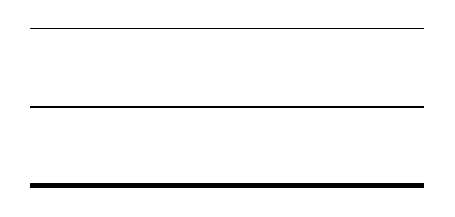
\begin{tikzpicture}
\draw (0,0)--(5,0);
\draw[line width = 1pt] (0,-1)--(5,-1);
\draw[line width = 2pt] (0,-2)--(5,-2);
\end{tikzpicture}
```

TikZ 的預設值是 0.4pt

###箭頭

可以利用 > 與 < 來指定箭頭的形式

```latex
\begin{tikzpicture}
\draw[-] (0,0)--(5,0);
\draw[<-] (0,-1)--(5,-1);
\draw[->] (0,-2)--(5,-2);
\draw[<->] (0,-3)--(5,-3);
\draw[|->] (0,-4)--(5,-4);
\draw[|<->|] (0,-5)--(5,-5);
\draw[|-|] (0,-6)--(5,-6);
\draw[->|] (0,-7)--(5,-7);
\draw[>->>] (0,-7)--(5,-7);
\end{tikzpicture}
```

上圖是一些示範

###預定義好的樣式

TikZ 也有預先定義好一些樣式,讓我們可以使用

```latex
\begin{tikzpicture}
\draw[dotted] (0,0)--(5,0);
\draw[densely dotted] (0,-1)--(5,-1);
\draw[loosely dotted] (0,-2)--(5,-2);
\draw[dashed] (0,-3)--(5,-3);
\draw[densely dashed] (0,-4)--(5,-4);
\draw[loosely dashed] (0,-5)--(5,-5);
\end{tikzpicture}
```

###平移、縮放與旋轉

可以利用 shift 來達成平移的效果

```latex
\begin{tikzpicture}
\draw (0,0) rectangle (1,1);
\draw[shift={(2,0)}] (0,0) rectangle (1,1);
\draw[shift={(2,2)}] (0,0) rectangle (1,1);
\draw[shift={(0,2)}] (0,0) rectangle (1,1);
\draw[shift={(-2,2)}] (0,0) rectangle (1,1);
\draw[shift={(-2,0)}] (0,0) rectangle (1,1);
\draw[shift={(-2,-2)}] (0,0) rectangle (1,1);
\draw[shift={(0,-2)}] (0,0) rectangle (1,1);
\draw[shift={(2,-2)}] (0,0) rectangle (1,1);
\end{tikzpicture}
```

* 第二個正方形的左下頂點由 (0,0) 移到了 (2,0)
* 第三個正方形的左下頂點由 (0,0) 移到了 (2,2)
* 第四個正方形的左下頂點由 (0,0) 移到了 (0,2)
* 第五個正方形的左下頂點由 (0,0) 移到了 (-2,2)
* 第六個正方形的左下頂點由 (0,0) 移到了 (-2,0)
* 第七個正方形的左下頂點由 (0,0) 移到了 (-2,-2)
* 第八個正方形的左下頂點由 (0,0) 移到了 (0,-2)
* 第九個正方形的左下頂點由 (0,0) 移到了 (2,-2)

也可以在 shift 前加上 x 或 y 來決定平移的方向,但在這種情況下就不能使用內建的長度單位,需要自行指定

```latex
\begin{tikzpicture}
\draw (0,0) rectangle (1,1);
\draw[xshift=100pt] (0,0) rectangle (1,1);
\draw[xshift=-100pt] (0,0) rectangle (1,1);
\draw[yshift=100pt] (0,0) rectangle (1,1);
\draw[yshift=-100pt] (0,0) rectangle (1,1);
\end{tikzpicture}
```

旋轉則需要利用 rotate

```latex
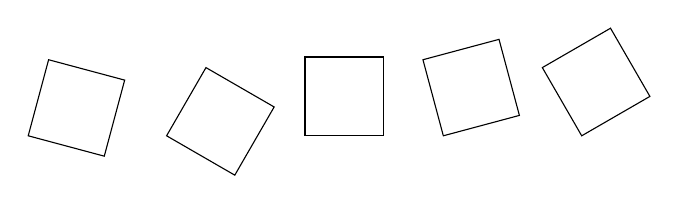
\begin{tikzpicture}
\draw (0,0) rectangle (1,1);
\draw[xshift=100pt, rotate=30] (0,0) rectangle (1,1);
\draw[xshift=50pt, rotate=15] (0,0) rectangle (1,1);
\draw[xshift=-100pt, rotate=-15] (0,0) rectangle (1,1);
\draw[xshift=-50pt, rotate=-30] (0,0) rectangle (1,1);
\end{tikzpicture}
```

\end{markdown}\newpage
\begin{markdown}
#30天 LaTeX 挑戰 Day 21 Ti*k*Z

-------

##進階使用

###節點

在 TikZ 中可以利用 `\node(name) at(x,y) {text};` 放置節點

```latex
\begin{tikzpicture}
\draw[help lines] (-2,-2) grid (2,2);
\node(1) at(0,0) {原點};
\end{tikzpicture}
```

想要連接兩個節點時,可以將座標改為兩個節點的名字

```latex
\begin{tikzpicture}
\node(A) at(0,0) {A};
\node(B) at(2,0) {B};
\node(C) at(0,2) {C};
\draw (A)--(B)--(C);
\end{tikzpicture}
```

`\node `如同 `\draw `也可以使用選項來調整樣式

```latex
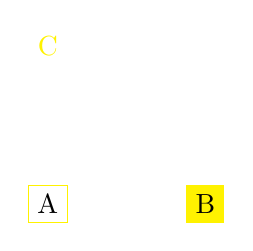
\begin{tikzpicture}
\node[draw=yellow](A) at(0,0) {A};
\node[fill=yellow](B) at(2,0) {B};
\node[text=yellow](C) at(0,2) {C};
\end{tikzpicture}
```

當然也有一些是只能用在 `\node `上的選項

```latex
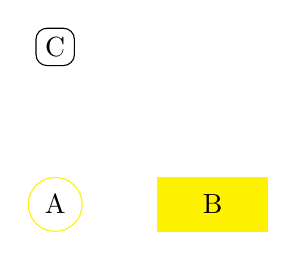
\begin{tikzpicture}
\node[draw=yellow,circle](A) at(0,0) {A};
\node[fill=yellow, minimum width=40pt, minimum height=20pt](B) at(2,0) {B};
\node[draw=black, rounded corners](C) at(0,2) {C};
\end{tikzpicture}
```

* 第一個節點用 circle 將外匡變成圓形的
* 第二個節點用 minimum width/height 定義節點的最小長寬
* 第三個節點用 rounded corners 把節點的邊角轉成圓角

但有時候我們並不想要直接把節點放到指定的座標,而是想放到該座標的上下左右,這個時候也可以利用 TikZ 內建的選項來達成

```latex

\begin{tikzpicture}
\node[left] at(0,0) {left};
\node[right] at(0,0) {right};
\node[above] at(0,0) {above};
\node[below] at(0,0) {below};
\draw[fill=black] (0,0) circle (.1);
\end{tikzpicture}
```

* 第一個節點在 (0,0) 的左邊
* 第二個節點在 (0,0) 的右邊
* 第三個節點在 (0,0) 的上方
* 第四個節點在 (0,0) 的下方

###自定義樣式

如果你圖片裡的節點畫線條都有相似的共同點,你可以在`\begin {tikzpicture}` 後加一個方括號,並將共通的選項放在方括號中

```latex
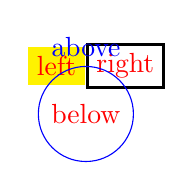
\begin{tikzpicture}[text = red]
\node[left, fill = yellow] at(0,0) {left};
\node[right, draw = black, line width =1pt] at(0,0) {right};
\node[above, text = blue] at(0,0) {above};
\node[below, draw = blue, circle] at(0,0) {below};
\end{tikzpicture}
```

如果你有一個很複雜的樣式,但又不是共通的,你可以利用`\tikzset{}`來將複雜的樣式定義成一個選項

```latex
\tikzset{mynode/.style = {
draw = gray!70!black,
line width = 0.8pt,
fill = blue!30,
rounded corners,
inner sep = 6pt, %文字與邊匡的距離
minimum width = 40pt,
minimum height = 20pt}
}
```

使用時只要用 `\node[mynode]` 即可

```latex
\begin{tikzpicture}[->, line width = 2pt]
\node[mynode] (1) at (0,0) {First Thing};
\node[mynode] (2) at (3,0) {Second Thing};
\node[mynode] (3) at (6,0) {Third Thing};
\draw (1)--(2);
\draw (2)--(3);
\end{tikzpicture}
```

這樣就方便許多了

###函數圖

畫函數一樣是使用`\draw ` 這個命令

```latex
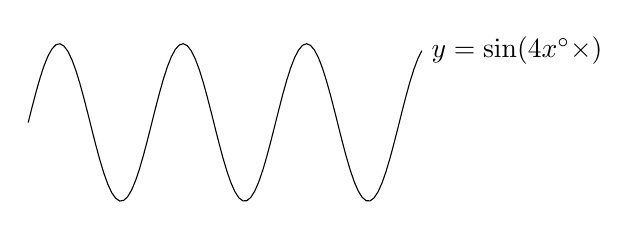
\begin{tikzpicture}
\draw[domain = 0:5, samples = 100] plot (\x,{sin(deg(\x*4))}) node[right] {$y=\sin(4x^\circ \times)$};
\end{tikzpicture}
```

domain 是我們要畫的區間,起點與終點要用冒號隔開,samples 決定圖形的精細程度,要特別注意的是需要運算的部分需要放在`{}`之間

![TikZ](TikZ)

上圖是可以使用的運算子,不過更複雜的函數圖形 TikZ 就很難畫出來了,所以下一篇會介紹 pgfplot 這個 package

\end{markdown}
\newpage
\begin{markdown}
#30天 LaTeX 挑戰 Day 22 pgfplots

------

pgfplots 是一個可以畫出複雜的三維圖表的強大 Package,需要注意的是這個 Package 是基於前面介紹過的 Ti*k*Z,所以在使用之前請記得要先使用 Ti*k*Z。

##簡介

在使用 pgfplots 之前我們需要先使用 tikzpicture 環境,之後再使用 pgfplots  提供的 axis 環境。

```latex
\begin{tikzpicture}
\begin{axis}
......
\end{axis}
\end{tikzpicture}
```

我們要將 pgfplots 提供的命令放在 axis 環境中,第一個要介紹的是 `\addplot[可選參數]{方程式}` 這個命令,大部分可選參數是與 Ti*k*Z 的可選參數相同,方程式則是與大部分程式語言的表達方式一樣。

```latex
\begin{tikzpicture}
\begin{axis}
\addplot[domain=-5:5, color=blue] {x^2};
\end{axis}
\end{tikzpicture}
```

使用完之後也請不要忘記在最後面加上 ;。

##二維圖形

###函數圖

第一個介紹的還是函數圖,簡單的範例上面展示過了,所以這裡會比較注重在介紹不同的可選參數。

```latex
\begin{tikzpicture}
\begin{axis}
\addplot[domain=-5:5, color=blue] {x^2};
\end{axis}
\end{tikzpicture}
```

這是上面所展示的陽春例子,我們可以在多加一個方程式讓他看起來好一點。

```latex
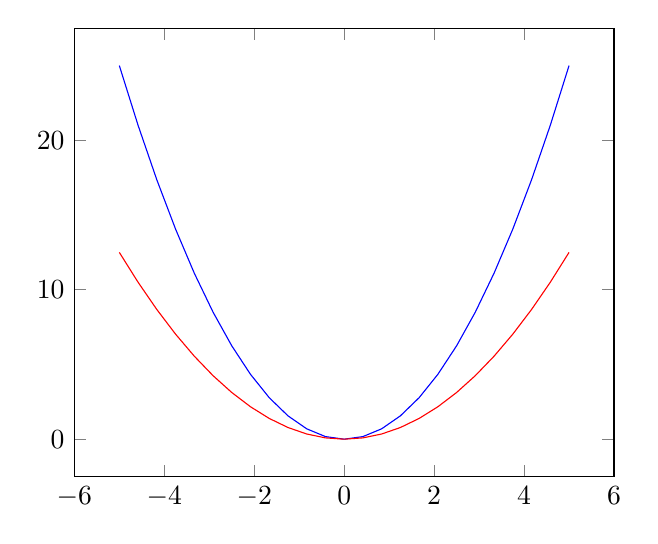
\begin{tikzpicture}
\begin{axis}
\addplot[domain=-5:5, color=blue] {x^2};
\addplot[domain=-5:5, color=red] {x^2/2};
\end{axis}
\end{tikzpicture}
```

可是這樣沒有標示難免會讓人搞混,所以我們可以利用 `\addlegendentry ` 加入註解。

```latex
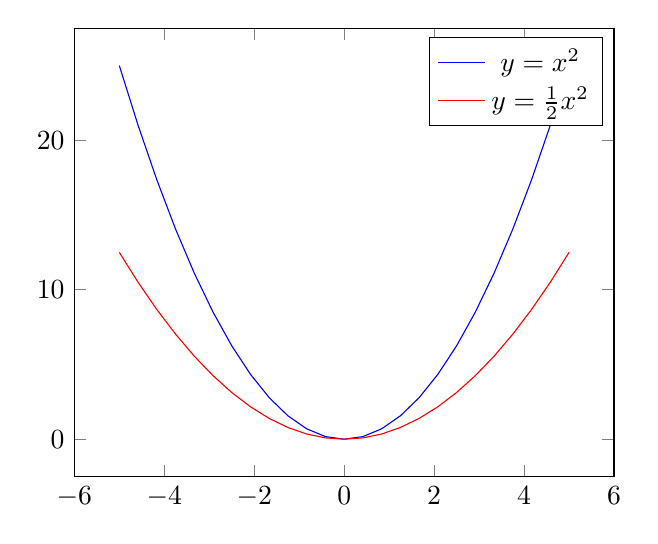
\begin{tikzpicture}
\begin{axis}
\addplot[domain=-5:5, color=blue] {x^2};
\addlegendentry{\(y=x^2\)}
\addplot[domain=-5:5, color=red] {x^2/2};
\addlegendentry{\(y=\frac{1}{2}x^2\)}
\end{axis}
\end{tikzpicture}
```

這樣就不會搞混了,如果今天想要用對數來當 x, y 軸的單位,pgfplots 也有提供 `\begin{semilogxaxis}` 與 `\begin{semilogyaxis}` 來解決這個問題。

```latex
\begin{tikzpicture}
\begin{semilogyaxis}
\addplot[domain=-10:10, color=blue, samples=1000] {log10(x)};
\end{semilogyaxis}
\end{tikzpicture}
```

有時候座標軸會不符合我們想要的樣式,這時可以利用 axis lines 來調整。

```latex
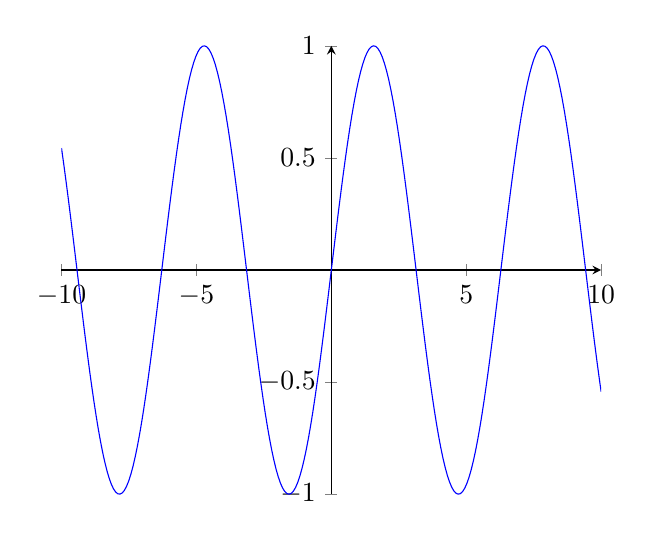
\begin{tikzpicture}
\begin{axis}[axis lines = middle]
\addplot[domain=-10:10, color=blue, samples=250] {sin(deg(x))};
\end{axis}
\end{tikzpicture}
```

\end{markdown}\newpage
\begin{markdown}
#30天 LaTeX 挑戰 Day 23 pgfplots

-----

###折線圖

除了函數圖外,pgfplots 也可以繪製折線圖。

```latex
\begin{tikzpicture}
\begin{axis}
\addplot coordinates{(0,0)(1,4)(2,3)(3,5)(4,2)(5,1)(6,0)(7,8)};
\end{axis}
\end{tikzpicture}
```

在 coordinates 後面的將放入所有折線圖的點,就可以畫出折線圖了,但有時座標軸上的標記與想像中的並不一樣,這時就需要用 xtick 與 ytick 調整。

```latex
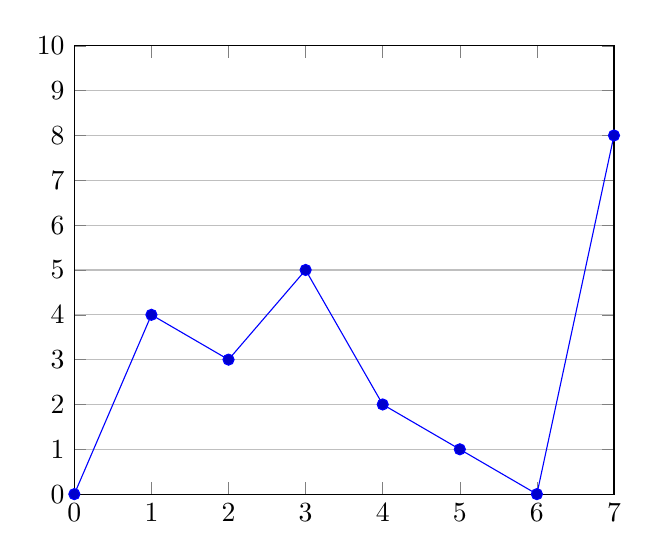
\begin{tikzpicture}
\begin{axis}[
xmin=0, xmax=7,
ymin=0, ymax=10,
xtick={0,1,2,3,4,5,6,7},
ytick={0,1,2,3,4,5,6,7,8,9,10},
ymajorgrids=true,
]
\addplot coordinates{(0,0)(1,4)(2,3)(3,5)(4,2)(5,1)(6,0)(7,8)};
\end{axis}
\end{tikzpicture}
```

* xmin, ymin, xmax, ymax 這些是指定 x 軸與 y 軸的最大、最小值
* xtick, ytick 是指定 x 軸與 y 軸上的標記的位置
* ymajorgrids 是繪製出與 y 軸相交的格線,可以用 xmajorgrids 來繪製出與 x 軸相交的格線,或用 grids=major 同時繪製兩者。

###長條圖

長條圖與折線圖有者異曲同工之妙

```latex
\begin{tikzpicture}
\begin{axis}[ybar, ybar interval=0.75, enlargelimits=0.1]
\addplot coordinates{(2040,9.50)(2030,10.60) (2020,12.58)};
\addplot coordinates{(2020,17.50) (2030,24.10) (2040,30.60)};
\legend{0~14歲人口所占比率(\%),65歲以上人口所占比率(\%)}
\end{axis}
\end{tikzpicture}
```

* ybar 指的是長條與 y 軸平行,另外還有 xbar 這個選項可以用。
* ybar interval 是指定長條之間的空隙,1 代表沒有空隙。
* enlarge limits 是調整整個座標軸與圖表的元素間的距離,另外也可以用enlarge x limits, enlarge y limits 等等來單獨調整特定的座標軸。

###散佈圖

散佈圖也很簡單。

```latex
\begin{tikzpicture}
\begin{axis}
\addplot[scatter, mark=*, only marks]
coordinates{(143,62) (50,594) (165,53) (139,348) (145,194) (75,533) (51,258) (154,492)};
\end{axis}
\end{tikzpicture}
```

* scatter 是讓顏色依據 y 軸的數值而變化
* only marks 是不讓點之間用線連起來
* mark 是指定點的標記的樣式

###從其他檔案輸入數據

上面的方法這只適用於數據只有寥寥幾筆時,不然如果有一千多筆,一個一個 key 未免太過勞神費力,不過 pgfplots 都幫你想好了,他可以讓你從 .dat 或 .csv 檔中輸入數據。

```latex
\begin{tikzpicture}
\begin{axis}[x tick label style={/pgf/number format/1000 sep=},width=10cm, grid=major]
\addplot table [x=year, y=youth, col sep=comma, mark=none] {data.csv};
\addlegendentry{0~14歲人口所占比率(\%)}
\addplot table [x=year, y=old, col sep=comma, mark=none] {data.csv};
\addlegendentry{65歲以上人口所占比率(\%)}
%\addplot table[meta=mid]{output.dat};
\end{axis}
\end{tikzpicture}
```

* x tick label style 是調整 x 軸上標示的樣式。
* table 是表示資料來源是類似表格的形式。
* x=, y= 是指定 x, y 的數據要從哪一欄輸入。
* col sep 是告訴 pgfplots 欄與欄的分界是用什麼符號。

##三維圖形

終於進入三維圖形了,

\end{markdown}\newpage
\begin{markdown}
#30天 LaTeX 挑戰 Day 24 用 Beamer 做簡報

------

如果想要用 LaTeX 製作簡報,可以利用 beamer 這個文件類型來製作,不只可以做差一張張的靜態投影片,也可以創造出一點點的動畫效果

##基礎使用

一個簡單的 beamaer 範例

```latex
\documentclass{beamer} %使用 beamer 為文件類型
\usepackage{xeCJK}
\setCJKmainfont{TW-Kai}
\author{Si manglam}
\title{如何使用 Beamer}
\subtitle{Beamer 大作戰}
\institute{IT 邦幫忙}
\date{2022/09/10}
\begin{document}
\begin{frame}
\titlepage
\end{frame}
\begin{frame}
\frametitle{標題}
\end{frame}
\end{document}
```

* frame 環境創造了新的投影片,所有要在投影片上的內容都要在這個環境內
* \titlepage 自動輸出標題頁
* \frametitle 	為當前投影片加入標題

如果作者並不只有一個人且來自不同機構,我們需要用微調來讓投影片更美觀

```latex
\title[重大發現]{一個足以改變人類未來的重大發現}
\author[Luke \& manglam]{Si manglam\inst{1} \and Luke\inst{2}}
\institute[實驗室、知名大學]{\inst{1}不具名的實驗室 \and \inst{2}某間知名大學}
\date[22xx 知名會議]{22xx/xx/xx某知名會議}
```

上面的例子中,兩個作者與兩個機構中間都用`\and ` 隔開,方括號內的則是在其他地方顯示的,現在可能還看不出差別,但看到下面用 `\usetheme{}` 來使用 beamer 內建主題的範例就可以看出明顯的差異了

```latex
\usetheme{Madrid}
\begin{document}
\begin{frame}
\titlepage
\end{frame}
\begin{frame}
\frametitle{標題}
\end{frame}
\end{document}
```

可以看到這樣美觀了許多,同時方括號的內容顯示在下面那排,更多的主題可以在<連結>中找到

##小技巧

beamer 與一般的文件一樣可以用`\tableofcontents `來建立目錄

<圖片>

也可以利用`\tableofcontents[currentsection]`來明確的標示現在的章節

<圖片>

beamer 也有針對投影片用途新定義一些環境

```latex
\begin{block}{這是一個 block}
文字
\end{block}

\begin{alertblock}{特別注意}
文字文字文字文字文字
\end{alertblock}

\begin{examples}
文字文字文字文字文字
\end{examples}
```

雖然 beamer 的主題有限,但只要換個色系就不會有人發現了

```latex
\usetheme{Madrid}
\usecolortheme{seahorse}
```

##overlay

利用`\only<頁數>{}`與`\discover<頁數>{}`可以控制元素出現的時機,兩者差別在一個是只在特定頁數出現,一個是隱形且只會在特定頁數出現。

```
\begin{center}
A\only<1>{第一頁出現}\\
A\discover<1-2>{第一、二頁}\\
A\only<2-3>{第二、三頁}\\
A\discover<3>{第三頁}\\
\end{center}
```

如果是想要讓條列的內容一條條出現可以直接在用`\begin{itemize}[<+->]`

```latex
\begin{itemize}[<+->]
\item 一
\item 二
\item 三
\end{itemize} 
```

但如果要特別指定頁數,就要在`\item `後加 <頁數>

```latex
\begin{itemize}[<+->]
\item<1-> 一
\item<2> 二
\item<3-4> 三
\item<4> 四
\item<5> 五
\end{itemize} 
```

可以看到有三出現在兩頁,這些就是 beamer 如何控制 Overlay。

\end{markdown}\newpage
\begin{markdown}
#30天 LaTeX 挑戰 Day 25 biblatex

------

biblatex 是一個管理參考文獻的 package,他可以幫助我們方便快速的管理參考文獻。

##前置作業

首先我們需要準備 .bib 檔, .bib 檔的基礎形式如下

```latex
@Article{key,
author = {作者},
title = {標題},
journal = {期刊},
year = {年份},
}
```


`@Article` 是宣告參考文獻是期刊中的文章,key 是在文章中引用連結使用的,但通常我們不用親自撰寫 .bib 檔,因為像 Google Scholar 之類的文獻資料庫都會提供 bibtex 的格式。

圖片

上圖是如何在 Google Scholar 取得 .bib 檔的方式。

##基礎使用

在準備好 .bib 檔後就可以開始使用 biblatex 了,首先我們需要告訴 biblatex 我們的 .bib 檔叫什麼名字。

```latex
%\usepackage{biblatex}
\addbibresource{name.bib}
```

利用 `\addbibresource{•}` 告訴 biblatex .bib 檔的名稱後,我們就可以利用 `\cite{key}` 在文章中引用參考文獻了。

```latex
Free software 跟價錢並沒有關係,這裡的 Free 指的是自由。\cite{stallman2002free}
```

如果不是使用 overleaf 的人需要注意,我們需要額外跑一次 bibber 和兩次 LaTeX,順序如下:

1. LaTeX
2. biber
3. LaTeX 
4. LaTeX

這樣就可以引用參考文獻了,但我們還需要用 `\printbibliography` 將有用到的參考資料都列出來。

```latex
\printbibliography
```

這樣所有被引用過的資料就都被列出來了,如果有參考文獻沒有被直接引用,又想要讓他出現在此,需要用 `\nocite{key}` 將他列出來。

```latex
Free software 跟價錢並沒有關係,這裡的 Free 指的是自由。\cite{stallman2002free}
\nocite{key}
\printbibliography
```

如果想將檔案中所有的參考文獻都列出,只需將 key 換成 * 就好了,如果引用了許多文章,但最後在列出時想要分類這一大群的參考文獻時,有兩種方法,第一種是利用 `type=` 來依照參考文獻的類型分類。

```latex
\printbibliography[type=article, title=article]
\printbibliography[type=book, title=book]
```

第二個方法是在撰寫 bib 檔時加入 `keywords` ,以便分類。

```latex
\printbibliography[keyword=LaTeX, title=article]
\printbibliography[keyword=Overleaf, title=book]
```

```latex
@book{stallman2002free,
  title={Free software, free society: Selected essays of Richard M. Stallman},
  author={Stallman, Richard},
  year={2002},
  publisher={Lulu. com},
  keywords={}
}
```

如果想要更進一步的了解 biblatex 到底可以做什麼,可以參考以下幾篇文章。

\end{markdown}\newpage
\begin{markdown}
#30天 LaTeX 挑戰 Day 26 animate

------

有時候人總是要會一兩招華而不實的招數,好在需要的時候秀一手,我們可以藉由在 pdf 中加入 gif 動畫以達到上述的效果。

##基礎使用

在使用之前需要先在導言區載入 graphicx package,在載入之後我們就可以利用 `\animategraphics{}{}{}{}` 來插入動畫,但在插入動畫之前,我們需要先了解 animate 是如何插入動畫的,實際上 animate 並不能將 gif 直接塞入 pdf 中,他是利用 javascript 讓 pdf 中的圖片可以動起來,所以在拿到 gif 後我們還需要將 gif 轉成其他格式。

###格式轉換

我們需要使用各種手段將 gif 轉換成 png 或 jpeg 等,可以使用 ImageMagick 這個工具來轉換,在安裝好之後可以在終端機用 convert 命令來轉換格式,

```
convert input.gif -coalesce output.png
```

可以利用這行命令將 gif 改成一系列的圖片。

###正式使用

```latex
\animategraphics[autoplay]{.5}{A-}{1}{5}
```

* 前面中括號內放可選參數
* 第一個花括號是指定動畫的幀數
* 第二個花括號是檔案的前綴名
* 第三個花括號是檔案的開頭、第四個則是結束,這條指令會將 A-1, A-2, A-3, A-4, A-5 作為動畫的

這裡有一系列的可選參數

* autoplay: 當滑到動畫所在的頁面時自動播放
* loop: 不斷重複播放動畫
* palindrome: 在動畫播放完後倒帶動畫,並重新循環
* step: 將動畫的放映模式改成點一下播一張
* controls: 決定動畫下的播放按鈕
* label: 給定一個 javascript 的標籤

###自行繪製

隨意使用網路上的 gif 圖可能會有版權相關的問題,但好在我們可以利用 animateinline 環境來自行繪製。

```latex
\begin{animateinline}[begin={\begin{tikzpicture}\draw (-1,-1) rectangle (3.5,1);}end={\end{tikzpicture}}]{0.5}
\draw (0,0)--(0.5,0);
\newframe
\draw (0,0)--(1,0);
\newframe
\draw (0,0)--(1.5,0);
\newframe
\draw (0,0)--(2,0);
\newframe
\draw (0,0)--(2.5,0);
\newframe
\draw (0,0)--(3,0);
\newframe
\draw (0,0)--(3.5,0);
\end{animateinline}
```

* begin 跟 emd 是指在每一幀之前自動插入的命令
* 整個動畫的大小是依據第一幀的大小來進行縮放的,所以我在每一幀都加入了看不見的正方形以維持動畫大小的一致性

當然這些只是簡單的範例,只要你想得到,沒有什麼是你做不出來的。


\end{markdown}\newpage
\begin{markdown}
#30天 LaTeX 挑戰 Day 27 lualatex

------

Lualatex 是將 Lua 與 TeX 結合在一起,讓改動 TeX 的排版規則時可以不用 TeXing,更詳細的使用需要對 LuaTeX 與 LaTeX 有深刻的認識,目前我的能力還不到這麼深厚,所以我只介紹一些基礎的用法。

## 基礎用法

想要在 LuaLaTeX 裡使用 Lua 需要透過 `\directlua{}` 的協助,這個命令會將花括號中命令轉給 Lua 解釋器,要想讓 Lua 產出的結果可以轉回給 LaTeX 需要用 `tex.sprint`。

```lua
tex.sprint("$\cos(0)$等於".. math.cos(math.rad(0)))
```

執行之後可以看到 $\cos$ 被輸出出來了,這就是基礎的 LuaLaTeX 的用法更進階的也可以將 for 迴圈帶入使用

```lua
\directlua{
tex.sprint("\\begin{tabular}{|c|c|c|}")
tex.sprint("\\hline")
tex.sprint("x & sin(x) & cos(x) \\\\ ")
tex.sprint("\\hline")
for x = 0,180,10 do
	tex.sprint(x .." & ".. math.sin(math.rad(x)) .." & ".. math.cos(math.rad(x)) .." \\\\ ")
	tex.sprint("\\hline")
end
tex.sprint("\\end{tabular}")
}
```

執行後可以看到有表格被產出了,如果有什麼重複性高的指令,也可以用這種方式來節省時間,這是基礎的 LuaLaTeX 的使用方法。

## 進階使用

進階使用我也不會所以在這裡放一個我看到的例子:

```lua
function fadelines(head)
        GLYPH = node.id("glyph")
        WHAT = node.id("whatsit")
        COL = node.subtype("pdf_colorstack")
        colorize = node.new(WHAT,COL)
        cvalue = 0
        for line in node.traverse_id(GLYPH,head) do
            colorize.data = cvalue.." "..1 - cvalue.." .5".." rg"
            node.insert_before(head, line, node.copy(colorize))
            cvalue = math.min(cvalue + .0008, 1)
        end
        return head
    end

    luatexbase.add_to_callback("pre_linebreak_filter", fadelines, "fadelines")
```

這樣產生的結果如下圖:

要達成這種效果,需要對 LuaLaTeX 以及 LaTeX 有著即為深厚的認識。

\end{markdown}\newpage
\begin{markdown}
#30天 LaTeX 挑戰 Day 28 用 LuaLaTeX 做動畫

-----

繼上一篇介紹了 LuaLaTeX 後,相信大家都瞭解了 LuaLaTeX 的基本使用方式,今天要教大家的則是如何用 LuaLaTeX 加上 animate 製作動畫,特別提醒:這不是正常的 LuaLaTeX 的使用方法。

## 基礎創作

基本上最常使用到的環境大概是物件的移動,我們不太可能一幀幀的繪製出物件的移動軌跡,因為那樣程式碼會顯得過於冗長,所以我們可以利用 for 迴圈去縮減程式碼。

```lua
\begin{luacode}
tex.sprint("\\begin{animateinline}[autoplay,loop]{10}")
for x = -4,4,0.1 do
	tex.sprint("\\begin{tikzpicture}")
	tex.sprint("\\draw[color=white] (-5,-5) rectangle (5,5);")
	tex.sprint("\\draw[fill=black] (".. x ..",0) circle (0.5);")
	tex.sprint("\\end{tikzpicture}")
	tex.sprint("\\newframe")
end
tex.sprint("\\end{animateinline}")
\end{luacode}
```

編譯出來的動畫是一個小球漸漸的從左移到右,比起一幀幀繪製,這樣簡單多了。

## 進階創作

更進階的創作用法可以再加上 if 迴圈,例如以下的動畫:

```lua
\begin{luacode}
tex.sprint("\\begin{animateinline}[autoplay,loop]{10}")
for x = 0,360,5 do
	tex.sprint("\\begin{tikzpicture}")
	tex.sprint("\\draw[color=white] (-2,-2) rectangle (2,2);")
	if (math.sin(math.rad(x)) > 0) then
		tex.sprint("\\draw[fill=red] (0,".. math.sin(math.rad(x)) ..") circle (0.5);")
	else
		tex.sprint("\\draw[fill=blue] (0,".. math.sin(math.rad(x)) ..") circle (0.5);")
	tex.sprint("\\end{tikzpicture}")
	tex.sprint("\\newframe")
end
tex.sprint("\\end{animateinline}")
\end{luacode}
```

編譯出的結果是一個會隨著高度變換顏色的小球,更多的使用方法就要靠你們自己去發想了,只要是有規律地動會,都可以用這種方式繪製出來的。

\end{markdown}\newpage
\begin{markdown}
#30天 LaTeX 挑戰 Day 29 etoolbox

-------

倒數第二天了,今天要跟大家介紹 etoolbox 這個可以讓你編輯已有命令的 package。

##使用之前

因為這個 package 是讓你編輯已有命令,所以在編輯之前我們必須先找出命令的原始定義,LaTeX 提供了 `\show` 這個命令來協助我們,只要在 `\show `後面接上想要查詢的指令就在 .log 檔中看到命令的定義,除了利用`\show `查詢之外,我們也可以直接到檔案的原始碼尋找。

除了 `\show `之外,我們也可以利用

###



\end{markdown}\newpage
\begin{markdown}
#30天 LaTeX 挑戰 Day 30 繼續前行

-----

30 天的鐵人賽長跑來到了最後一天,今天就不再寫技術相關的內容了,而要來介紹哪裡可以找到更多關於 LaTeX 的資料,

##網頁

以下幾個網頁是我很推薦的資料來源

* CTAN
* Overleaf
* Stack Exchange

CTAN 是 Comprehensive TeX Archive Network 的縮寫,基本上只要是 TeX 有關的資料都會被收藏在此(LaTeX 當然也被包含在內),如果有什麼 package 或使用手冊想要找,甚至是自己寫了一個 package 想要與全世界的 TeX 使用者共享,只要到 CTAN 就對了。

Overleaf 不只提供了線上編譯 LaTeX 的服務,他們也為了推廣 LaTeX 寫了許多的技術文章,最棒的是他們的技術文章是為了初學者而設計的,所以不用怕看不懂,但想當然的內容是用英文寫的。

大部分人應該都聽過 Stack Exchange ,如果你有什麼問題想問,不仿先來這裡看看有沒有人問過。

##書籍

書籍有以下幾本

* The TeX book
* The Not So Short Introduction to LATEX2ε
* 簡單高效 LaTeX
* 大家來學 LaTeX

The TeX Book 是由高德納教授親自編寫的書籍,可以說是

\end{markdown}\newpage
\setlength{\parindent}{20pt}
\begin{markdown}
#30天 LaTeX 挑戰 Day 31 Beyond LaTeX

-------

30 天的挑戰終於過去了,我也算是用另一種方式成為了勇者,當初會想寫下這系列的文章可說全部都是意外,事情得要從一個地科作業開始說起,當時在寫地科作業的我正被「如何在 page 內加入數學方程式」而困擾著,於是我打開了 page 內建的插入方程式功能,只見一行大字出現在視窗內「請使用 mathml 或 LaTeX 來插入數學方程式」,這就是我遇見 LaTeX 的過程。

後來我就開始學習 LaTeX ,在學習的過程中我發現跟 LaTeX 有關的中文資料只有兩種,不是簡體字就是有一定年份的資料,除了這之外就全部都是英文資料了,雖然雙語能力固然重要,但沒有中文資料真的太慘了,所以我就下定決心要留點資料,那時剛好看到了鐵人賽,於是便下定決心要做這件事情。

\end{markdown}

\end{document}